 \chapter{Resultados e Discussões}\label{cap:resultados}


Este estudo conta com a realização de testes nas bases de dados da UCI Machine Learning\footnote{http://archive.ics.uci.edu/ml/} - um repositório de dados a serviço da comunidade de aprendizado de máquina criado por estudantes de pós-graduação na UC Irvine em 1987 e que é utilizado por educadores e pesquisadores como fonte primária de aplicações de aprendizado de máquina. 

%* lembrar que as bases são essas (iris, ...) por serem já estudadas, e de prévio conhecimento, onde a partir de estudos em bases assim pode-se ter resultados conclusivos e expandir para outras bases. É como se testase com base conhecida para depois pegar uma nova.


 
As bases de dados escolhidas para este trabalho foram: Seeds, Iris, Glass, Wine. Essas bases são bastante utilizadas em vários trabalhos\footnote{https://archive.ics.uci.edu/ml/datasets/glass+identificpation, https://archive.ics.uci.edu/ml/datasets/iris, https://archive.ics.uci.edu/ml/datasets/wine, https://archive.ics.uci.edu/ml/datasets/seeds}  e por meio deles há possibilidade de análise de seus comportamentos mediante resultados, visto que todas as bases são classificadas e já possuem seus grupos definidos, servindo de referência para comparar os resultados desta pesquisa, sem esquecer que o trabalho é com os \textit{clusters} já formados e não na formação deles. Outro motivo desta seleção das bases é mitigar ao máximo a utilização das técnicas de \textit{Feature Engineering} \cite{Casari2018}, que são técnicas de manipulação de dados empregadas na base para aplicação do algoritmo de aprendizado de máquina utilizado na fase de preparação dos dados.


As tabelas apresentadas como resposta dos algoritmos de rotulação para cada base de dados possuem o seguinte formato: a primeira coluna (\textbf{Cluster}) é um número que representa cada cluster de forma sequencial; a segunda coluna (\textbf{Rótulos}) é representada pelo par \textbf{Atributo} e \textbf{Faixa}, o qual define o rótulo do cluster respectivo, podendo haver ou não mais atributos para compor o rótulo; a coluna \textbf{Relevância} tem a importância de informar o quanto, em porcentagem, aquele atributo é relacionado aos demais na definição do rótulo daquele \textit{cluster}. A quinta coluna, \textbf{Fora da Faixa}, exibe o erro em quantidade de elementos que não estão naquela faixa definida naquele rótulo e, por último, a \textbf{Acurácia Parcial}, que exibe, em porcentagem, o valor de acertos dos elementos que são representados pelo atributo e faixa da respectiva linha. 

A obtenção da acurácia dos \textit{clusters} só é possível porque as bases de dados já possuem seus grupos definidos, por conseguinte, há o conhecimento de quais elementos fazem parte de um determinado grupo. Dessa maneira, qualquer resultado da aplicação dos algoritmos nos \textit{clusters} pode ser confrontado com as informações dos \textit{clusters} inicialmente retirados da UCI Machine Learning e, assim, poderá ser calculada a porcentagem de acertos. 

A divisão deste capítulo iniciará por uma explanação da implementação do trabalho explicando as ferramentas utilizadas no desenvolvimento com configurações de algumas variáveis e cada seção se referirá a uma base de dados utilizada, sendo esta dividida em subseções para os seguintes algoritmos: Naive Bayes, CART e KNN.

\section{Implementação}\label{cap:resultados:sec:implement}



Para gerar os resultados aqui descritos, foram realizadas implementações utilizando-se a ferramenta MATLAB\footnote{http://www.mathworks.com/products/matlab/ ; versão: R2016a(9.0.0.341360); 64-bit (glnxa64)}, sendo possível utilizar suas funções de aprendizado de máquina já implementadas na \textit{Statistics and Machine Learning Toolbox} . Por apresentar linguagem técnica e funções já prontas direcionadas para aprendizado de máquina,essa ferramenta foi selecionada para colocar em prática essa pesquisa.

Ao longo da pesquisa foram realizados vários testes, porém, houveram alterações de algumas variáveis e métodos de discretização, sempre com o objetivo de obter os melhores resultados. As variáveis e métodos alterados são: variância (${V}$), número de faixas (${R}$), e tipo de discretização, ${TipoDiscretização}$ (EWD,EFD). 

Ao longo da pesquisa foram realizados vários testes, porém, houve alterações de algumas variáveis e métodos de discretização, sempre com o objetivo de obter os melhores resultados. As variáveis e métodos alterados são: variância (${V}$), número de faixas (${R}$) e tipo de discretização (EWD,EFD). 

%Fazendo um breve resumo sobre as configurações das variáveis, a variação ${V}$ existe para evitar a ambiguidade dos rótulos, ou seja, quando os rótulos apresentarem os mesmos resultados: atributo e faixa de valor. O número de faixas (${R}$), é o número de faixas definido de forma que os atributos tenham seus valores mapeados de acordo com o valor da variável, e dependendo de como os dados do atributo são dispostos, existirá uma melhor divisão no número de faixas \footnote{Apêndice \ref{apendice:1}}, contudo, os resultados foram realizados com ${R=3}$ em concordância ao trabalho de \citeonline{Lopes2016} que também utilizou esse configuração, e assim podendo haver uma comparação entre resultados. Uma vez definido o número de faixas será escolhido qual método de discretização será aplicado (EWD,EFD), decidindo qual faixa cada valor irá ficar.  

Fazendo um breve resumo sobre as configurações das variáveis, a variação ${V}$ existe para evitar a ambiguidade dos rótulos, ou seja, quando os rótulos apresentarem os mesmos resultados: atributo e faixa de valor. O número de faixas (${R}$) é definido de forma que os atributos tenham seus valores mapeados de acordo com a faixa de valor correspondente e, uma vez definido o número de faixas será escolhido qual método de discretização será aplicado (EWD,EFD), decidindo-se com qual faixa cada valor irá ficar.



%Além de evitar a ambiguidade dos rótulos a variável ${V}$ pode ser utilizada também para selecionar mais de um atributo para ser o rótulo do cluster. 


%A utilização da variação ${V}$ para escolha de rótulos acontece após uma análise da tabela de correlação dos atributos (seção \ref{cap:ferramentas:sec:tecnica}), a exemplo da tabela \ref{tab:matrelevancia:seeds:nb}. E existindo valores muito próximos em relação a outros (cabe a uma análise se necessário), poderá utilizar esses atributos também como rótulos para melhor definir o cluster. A variável ${V}$ pode ser configurada com um valor que possa abranger esses atributos que possuam valores de porcentagens próximos ao do atributo de maior valor na tabela (mais relevante). O valor de ${V}$ é subjetivo e sua adição é condicionada a análise da aplicação do algoritmo na bases de dados.

%É importante ressaltar a criação da tabela de correlação de atributos (Matriz de Atributos Importantes). Essa tabela é implementada conforme a técnica de correlação entre atributos com algoritmos supervisionados, seção \ref{cap:ferramentas:ssec:algsuper}, onde cada célula da tabela é preenchida através da execução de um algoritmo supervisionado. Estas execuções são realizadas em todos os atributos da cada cluster existente na base de dados.

%Após a tabela preenchida, o atributo rótulo será selecionado a partir do maior valor em relação aos outros atributos do grupo, que é representado pela linha da tabela (matriz de atributos). Também poderá ser selecionado como rótulo os atributos que possuam o valor entre a diferença de ${V}$ com o atributo de maior valor (mais relevante). Por exemplo, se o valor de ${V=5\%}$ e o atributo de maior valor é \textbf{95\%}, então todos os atributos que possuírem o valor a partir de \textbf{90\%} serão considerados rótulos também.

%a cada iteração do algoritmo é preenchida uma célula da tabela com o valor de correlação do primeiro atributo até o último atributo de um cluster, e depois iniciado o mesmo procedimento a outro cluster até não haver mais clusters. Após a tabela estar montada o atributo rótulo será selecionado a partir do maior valor em relação aos outros atributos do grupo, e caso seja necessário também é selecionado como rótulo os atributos que possuam o valor entre a diferença de ${V}$ com o atributo de maior valor (mais relevante). 


%A cada base de dados descritas nas seções seguintes, são configuradas algumas variáveis, método de discretização e implementado dois algoritmos de aprendizado supervisionado com paradigmas diferentes para fazer rotulação. Cada algoritmo terá como resultado o rótulo por cluster de dados.


\section{Base de Dados 1 - Seeds - Identificação de Tipos de Semente}
Essa base é composta por sete  atributos definindo suas características e mais um: a  classe, que é responsável por identificar os tipos de sementes \cite{Charytanowicz2010}. Esses elementos foram construídos a partir de sete parâmetros geométricos medidos dos grãos de trigo: \textit{area} - A, \textit{perimeter} - P, \textit{compactness} - C, \textit{length of kernel} - Lkernel, \textit{width of kernel} - Wkernel, \textit{asymmetry coefficient} - asymetry, \textit{length of kernel groove} - lkgroove.

Os valores dos atributos são todos contínuos e não existem valores em branco, possuindo um total de 210 registros classificados em três categorias bem distribuídas entre as classes, definindo-se estas como base de dados balanceada, por conta dessa distribuição dos registros: 
\begin{itemize}[noitemsep]
 \item 70 elementos do tipo \textit{Kama};
 \item 70 elementos do tipo \textit{Rosa};
 \item 70 elementos do tipo \textit{Canadian}.
\end{itemize}

Para classificar as sementes como \textit{Kama}, \textit{Rosa} e \textit{Canadian}, foi utilizada uma técnica de raio X que é relativamente mais barata que outras técnicas de imagem, como microscopia ou tecnologia a laser. O material foi colhido de campos experimentais, explorados no Instituto de Agrofísica da Academia Polonesa de Ciências em Lublin.

As tabelas com os resultados dos rótulos apresentadas a seguir (tabelas \ref{tab:rot:seeds:nb},\ref{tab:rot:seeds:cart}, \ref{tab:rot:seeds:knn}) exibem os resultados de rotulação dos algoritmos Naive Bayes, CART e KNN, respectivamente, e no caso dos \textit{clusters}, cada linha determina um grupo: (1) \textit{Kama}, (2) \textit{Rosa} e (3) \textit{Canadian}. Como já mencionado neste capítulo, na seção \ref{cap:resultados:sec:implement}, antes de executar o algoritmo, algumas configurações são necessárias para executar o algoritmo, como a do método de discretização do tipo EFD, e também a divisão dos valores dos atributos em faixas com ${R=3}$ para todos os atributos e variação ${V=0\%}$ 

\subsection{Naive Bayes} \label{cap:resultados:ssec:seed:nb}

Na tabela \ref{tab:rot:seeds:nb} pode-se verificar o resultado da aplicação do algoritmo e através dela percebe-se que o pior rótulo foi no \textit{cluster} 1 com acurácia de 70\%, e com isso deixa de representar nove registros no total de setenta amostras, mas nos outros dois \textit{clusters} a acurácia sobe para 88\% com um erro de nove registros, porém, os rótulos nestes \textit{clusters} são diferentes, coincidindo somente os  valores das colunas \textbf{Fora da Faixa} e \textbf{Acurácia Parcial}.

\begin{table}[!h]
\centering
\caption{Resultado da rotulação com o algoritmo Naive Bayes}
\label{tab:rot:seeds:nb}
\scalebox{0.8}{
\begin{tabular}{llcrcc}
\hline \hline
\multicolumn{1}{c}{\cellcolor[HTML]{FFFFFF}} & \multicolumn{2}{c}{Rótulos}                & \multicolumn{1}{r}{}               & & \\ \cline{2-3}
Cluster                                      & Atributos      & \multicolumn{1}{c}{Faixa} & \multicolumn{1}{c}{Relevância(\%)} & Fora da Faixa & Acurácia Parcial(\%) \\ \hline \hline
1                                            & Lkernel           & ] 5.357 $\sim$  5.826 ]   & 2.85\%                               & 21 & 70\% \\  \hline
2                                            & lkgroove           & ] 5.791 $\sim$  6.55 ]   & 8.57\%                               & 9 & 87.15\%\\ \hline
%\multirow{-2}{*}{2}                          & lkernel        & ] 5.826 $\sim$  6.675 ]   & 92\%                               & 6\\  \hline
3                                            & wkernel      & [ 2.63 $\sim$  3.049 ]   & 4.28\%                               & 9 & 87.15\% \\ \hline \hline
\end{tabular}
}
\end{table}



%Na última coluna, \textbf{Acurácia Parcial}, apresenta em porcentagem o grau de acerto, por \textit{cluster}, dos registros que são representados pelo rótulo. Essa acurácia é possível, visto que, na descrição do \textit{dataset} da  \textit{UCI Machine Learning}\footnote{repositório de dados de onde está a base de dados. https://archive.ics.uci.edu/ml/datasets/seed} já é definido que cada grupo possui 70 (setenta) registros, e quais elementos fazem parte de cada \textit{cluster}. Já em uma análise desta tabela, os valores da coluna Relevância tiveram valore baixos, contudo, uma referência da qualidade do rótulos é diante dos elementos que ficam fora da faixa indicando o grau de representatividade do rótulo.

A última coluna, \textbf{Acurácia Parcial}, apresenta em porcentagem o grau de acerto, por \textit{cluster}, dos registros que são representados pelo rótulo. Analisando-se a coluna \textbf{Relevância} da tabela \ref{tab:rot:seeds:nb} nota-se que os valores são baixos, contudo, uma vez escolhido o atributo rótulo o grau de confiabilidade passa a ser o número de erros do rótulo, pois quanto menores são os erros mais representabilidade possui o rótulo. Dessa forma, o menor valor de acurácia ficou em 70\% (setenta por cento) no \textit{cluster} 1, indicando que dentre as setenta amostras, 21 (vinte e um) não são representadas pelo rótulo, e nos outros \textit{clusters} acima de 87\% (oitenta e sete por cento).

Segue abaixo o resultado do algoritmo Naive Bayes na base de dados \textbf{Seeds} com seus rótulos: 
\begin{itemize}[noitemsep]
 \item ${r_{c_1}=\{ (Lkernel, ] 5.357 \sim  5.826 ]) \} }$  
 \item ${r_{c_2}=\{ (lkgroove, ] 5.791 \sim  6.55]) \} }$
 \item ${r_{c_3}=\{ (wkernel, [2.63 \sim  3.049])\} }$
\end{itemize}


\subsection{Classification and Regression Trees - CART}\label{cap:resultados:ssec:seed:cart}

Na tabela \ref{tab:rot:seeds:cart} que segue o mesmo modelo da tabela visto anteriormente e apresenta o resultado da aplicação do algoritmo supervisionado na base Seeds. O CART é utilizado pela toolbox do MATLAB como algoritmo de classificação de árvore de decisão. 
%O que se pretende fazer é seguir a pesquisa e testar a base de dados com um paradigma  diferente para fazer rotulação nos clusters.

\begin{table}[!h]
\centering
\caption{Resultado da aplicação do algoritmo CART}
\label{tab:rot:seeds:cart}
\scalebox{0.8}{
\begin{tabular}{llcrcc}\hline \hline

\multicolumn{1}{c}{\cellcolor[HTML]{FFFFFF}} & \multicolumn{2}{c}{Rótulos}                      & \multicolumn{1}{r}{}            \\ \cline{2-3}
Cluster                                      & Atributos      & \multicolumn{1}{c}{Faixa}       & \multicolumn{1}{c}{Relevância(\%)} & Fora da Faixa & Acurácia Parcial(\%)\\ \hline \hline
%                                             & area           & ] 12.78 $\sim$  16.14 ]         & 91\%          & 14 \\  
1                          & perimetro      & ] 13.73 $\sim$ 15.18 ]          & 5.71\%          & 14 & 80\%\\ \hline
2                          & lkgroove      & ]5.791 $\sim$   6.55 ]          & 5.71\%         & 9 & 87.15\% \\  \hline
3                          & perimetro        & [ 12.41 $\sim$  13.73 ]         & 4.28\%           & 5 & 92.8\%\\ \hline \hline
\end{tabular}}
\end{table}

%Os rótulos encontrados para cada cluster foi somente uma tupla (atributo/faixa) para cada grupo de dados, e coincidindo o mesmo resultado no \textit{cluster} 2 ao Naive Bayes visto anteriormente. Já nos outros rótulos, os mesmo com rótulos diferentes alcançaram acurácias melhores.

Analisando os rótulos encontrados percebe-se que as acurácias do CART são melhores aos do algoritmo visto anteriormente, e na coluna \textbf{Atributos} há uma repetição do \textbf{perimetro} em dois clusters: \textit{Kama} e \textit{Canadian}. Na situação apresentada na tabela \ref{tab:rot:seeds:cart} esses atributos repetidos não representam as mesmas amostras na base de dados, porque mesmo com o rótulo possuindo o mesmo atributo as faixas de cada atributo são diferentes tornando-os rótulos distintos.

O resultado da rotulação utilizando o algoritmo CART na base de dados \textbf{Seeds} tem como rótulos: 
\begin{itemize}[noitemsep]
 \item ${r_{c_1}=\{ (perimetro, ]13.73 \sim 15.18]) \} }$
 \item ${r_{c_2}=\{ (lkgroove, ] 5.791 \sim  6.55]) \} }$
 \item ${r_{c_3}=\{ (perimetro, [12.41 \sim  13.73])\} }$
\end{itemize}


\subsection{K-Nearest Neighbor - KNN} \label{cap:resultados:ssec:seed:knn}

Na tabela \ref{tab:rot:seeds:knn} exibe o resultado da aplicação do KNN na base Seeds e os rótulos encontrados são os mesmos do CART com uma diferença somente nos dados de relevância do atributo, o que não muda o grau de representatividade do rótulo. 
\newpage
\begin{table}[!h]
\centering
\caption{Resultado da aplicação do algoritmo KNN}
\label{tab:rot:seeds:knn}
\scalebox{0.8}{
\begin{tabular}{llcrcc}\hline \hline

\multicolumn{1}{c}{\cellcolor[HTML]{FFFFFF}} & \multicolumn{2}{c}{Rótulos}                      & \multicolumn{1}{r}{}            \\ \cline{2-3}
Cluster                                      & Atributos      & \multicolumn{1}{c}{Faixa}       & \multicolumn{1}{c}{Relevância(\%)} & Fora da Faixa & Acurácia Parcial(\%)\\ \hline \hline
%                                             & area           & ] 12.78 $\sim$  16.14 ]         & 91\%          & 14 \\  
1                          & perimetro      & ] 13.73 $\sim$ 15.18 ]          & 12.85\%          & 14 & 80\%\\ \hline
2                          & lkgroove      & ]5.791 $\sim$   6.55 ]          & 7.14\%         & 9 & 87.15\% \\  \hline
3                          & perimetro        & [ 12.41 $\sim$  13.73 ]         & 5.71\%           & 5 & 92.8\%\\ \hline \hline
\end{tabular}}
\end{table}

O resultado da rotulação utilizando o algoritmo KNN na base de dados \textbf{Seeds} tem como rótulos: 
\begin{itemize}[noitemsep]
 \item ${r_{c_1}=\{ (perimetro, ]13.73 \sim 15.18]) \} }$
 \item ${r_{c_2}=\{ (lkgroove, ] 5.791 \sim  6.55]) \} }$
 \item ${r_{c_3}=\{ (perimetro, [12.41 \sim  13.73])\} }$
\end{itemize}


\subsection{Comparativo entre Algoritmos na Base de Dados Seeds} \label{cap:resultados:ssec:compalgoritmos:seeds}
O CART e KNN foram dentre os três algoritmos, os que obtiveram os rótulos com melhores acurácias, que por sua vez tiveram os mesmos rótulos em todos os três grupos: \textit{Kama}, \textit{Rosa} e \textit{Canadian}. Analisando-se os resultados: o Naive Bayes no \textit{cluster} 1, ${r_{c_1}=\{ (Lkernel, ] 5.357 \sim  5.826 ]) \} }$, foi o que obteve maior número de elementos fora da faixa, isso quer dizer que no total de setenta amostras de dados no grupo, vinte e um ficaram de fora do rótulo, resultando na menor acurácia entre os três algoritmos que tiveram quatorze amostras cada um; no \textit{cluster} 2 os três algoritmos coincidiram os resultados dos rótulos com nove erros cada; e no \textit{cluster} 3 (\textit{Canadian}) mais uma vez CART e KNN tiveram rótulos com acurácias mais altas com número de erros iguais a cinco registros nos dois algoritmos, comparado com nove registros  do Naive Bayes.

Para compreender melhor a representatividade do rótulo nos \textit{clusters} foi posto alguns gráficos apresentando o comportamento da base de dados em relação a alguns atributos. Com estes gráficos é possível visualizar se o rótulo está de fato representando um determinado grupo. Os gráficos são dispostos em duas dimensões e o atributo referente a cada eixo foi escolhido para melhor representar a amostra.

O gráfico da figura \ref{fig:grafico_NB_cluster1_lkernel_lkgroove_seeds} contém uma relação dos atributos \textbf{Lkernel} com \textbf{lkgroove} e representa a amostra de dados dos três grupos: \textit{Kama}, \textit{Rosa} e \textit{Canadian}, contudo o objetivo deste gráfico é apresentar o comportamento do rótulo  no Naive Bayes, ${r_{c_1}=\{ (Lkernel, ] 5.357 \sim  5.826 ]) \} }$ no \textit{cluster} 1, e poder visualizar a representatividade do rótulo no grupo.

\begin{figure}[h!]
        \centering
        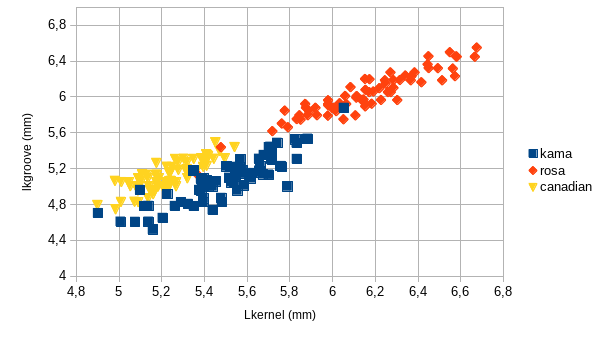
\includegraphics[scale=0.9]{figs/grafico_NB_cluster1_lkernel_lkgroove_seeds.png}
        \caption{Gráfico da disposição de elementos da Base Seeds entre os eixos \textbf{Lkernel} e \textbf{lkgroove}} \label{fig:grafico_NB_cluster1_lkernel_lkgroove_seeds}
\end{figure}

Na situação da figura \ref{fig:grafico_NB_cluster1_lkernel_lkgroove_seeds} , pode-se perceber que o grupo \textit{kama} (cluster 1) contém alguns erros, pois logo no início da faixa ${ (Lkernel, ] 5.357 \sim  5.826 ]) }$ é fácil visualizar que alguns dados  ficam fora da faixa indicando que não estão sendo representados pelo rótulo ocasionando os erros, contudo é possível ter uma impressão generalizada de todos os registros que o rótulo representa através dos valores de intervalo do rótulo. 

Na figura \ref{fig:grafico_NB_cluster1_2_wkernel_lkgroove_seeds} também apresenta a base Seeds distiguindo os grupos pelas formas geométricas: quadrados (\textit{Kama}), losango (\textit{Rosa}) e triângulos (\textit{Canadian}), mas com uma  relação entre  \textbf{lkgroove} e \textbf{wkernel} que  fazem parte dos resultados de rotulação do Naive Bayes no \textit{cluster} 2 ${r_{c_2}=\{ (lkgroove, ] 5.791 \sim  6.55]) \} }$ e no \textit{cluster} 3 ${r_{c_3}=\{ (wkernel, [2.63 \sim  3.049])\} }$.
 
\begin{figure}[h!]
        \centering
        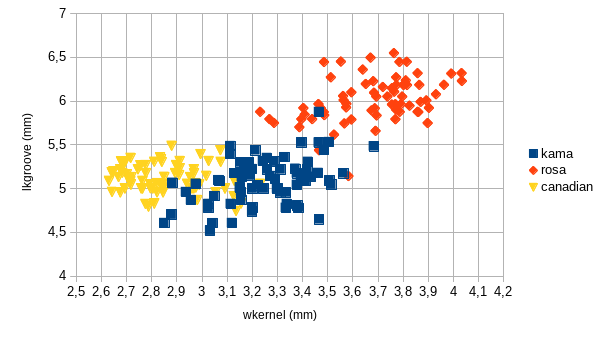
\includegraphics[scale=0.9]{figs/grafico_NB_cluster1_2_wkernel_lkgroove_seeds.png}
        \caption{Gráfico da disposição de elementos da Base Seeds entre os eixos \textbf{Lkernel} e \textbf{lkgroove}} \label{fig:grafico_NB_cluster1_2_wkernel_lkgroove_seeds}
\end{figure}
 
O atributo \textbf{lkgroove} faz parte do rótulo encontrado no grupo \textit{Rosa} (\textit{cluster} 2) pelo Naive Bayes, representado no gráfico pelo eixo Y da figura \ref{fig:grafico_NB_cluster1_2_wkernel_lkgroove_seeds} e sua faixa de dados é de fácil visualização no gráfico. Os valores do eixo Y acima de 5.791 até 6.55 são representados por ${r_{c_2}}$ do grupo Rosa figurado pelo losango no gráfico da figura \ref{fig:grafico_NB_cluster1_2_wkernel_lkgroove_seeds}. Já o ${r_{c_3}}$ possui o atributo \textbf{wkernel}  representado no gráfico no eixo X possuindo uma faixa de dados a partir de 2.63 até 3.049, e através desse intervalo é possível notar que há alguns dados não pertencentes ao ${r_{c_3}}$ do grupo Canadian. Com o gráfico fica fácil perceber que na disposição das amostras o grupo que mais se mistura  é o \textit{Kama}, implicando também na menor acurácia entre os rótulos. 


No outro gráfico, figura \ref{fig:grafico_CART_KNN_SEEDS_perimetro_lkgroove}, são relacionados dois eixos X e Y com os atributos \textbf{perimetro} e \textbf{lkgroove} respectivamente, e através desse plano cartesiano é possível identificar todos os grupos da base Seeds. Os dois algoritmos   CART e KNN possuem os mesmos resultados de rotulação para os três grupos mediante os dois atributos que estão representados no gráfico, dessa forma, com essa amostra de dados é possível representar o espaço de dados dos rótulos encontrados em cada algoritmo.

\begin{figure}[h!]
        \centering
        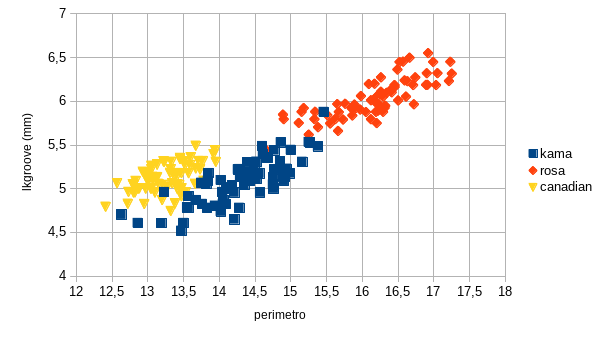
\includegraphics[scale=0.9]{figs/grafico_CART_KNN_SEEDS_perimetro_lkgroove.png}
        \caption{Gráfico da disposição de elementos da Base Seeds entre os eixos \textbf{Lkernel} e \textbf{lkgroove}} \label{fig:grafico_CART_KNN_SEEDS_perimetro_lkgroove}
\end{figure}

Os elementos do rótulo ${r_{c_1}=\{ (perimetro, ]13.73 \sim 15.18]) \} }$,  representam o grupo \textit{Kama}, que estão simbolizados de quadrados no gráfico, e através do atributo \textbf{perimetro} no intervalo de ]13.73 até 15.78] consegue-se visualizar no gráfico a amostra que o rótulo representa do \textit{cluster} 1 (\textit{Kama}), como também, alguns dados que não estão neste intervalo configurando os erros.

No \textit{cluster} 2 (\textit{Rosa}) figurando no gráfico como um losango pode-se perceber, através de seu rótulo ${r_{c_2}=\{ (lkgroove, ] 5.791 \sim  6.55]) \} }$, que o atributo \textbf{lkgroove} e seu intervalo estão bem definidos no gráfico. Qualquer valor no eixo Y no intervalo, a partir de 5.6791 até 6.55, é representado pelo rótulo ${r_{c_2}}$, mas mesmo com alguns erros visíveis na amostra, esse grupo foi o que ficou melhor delineado no gráfico e de fácil visualização para comprovar a representatividade dos rótulos encontrados pelos algoritmos CART e KNN. Já no \textit{cluster} 3 \textit{Canadian} não é diferente mediante ao rótulo encontrado pelos dois algoritmos ${r_{c_3}=\{ (perimetro, [12.41 \sim  13.73])\} }$. A partir da faixa do  ${r_{c_3}}$ no atributo \textbf{perimetro} as amostras representadas iniciam em 12.41 até 13.73,  mas mesmo no valor final do intervalo onde pode-se encontrar alguns erros, é possível mostrar que o ${r_{c_3}}$ consegue representar o grupo \textit{Canadian}.

\section{Base de Dados 2 - Iris - Identificação de Tipos de Plantas}

A base de dados Iris pertence a UCI Machine Learning, já usada em trabalhos como \citeonline{Lopes2016,Filho2015}, e utilizada em reconhecimento de padrões de plantas por lidar com classes bem definidas, pois contém 3 classes de 50 instâncias cada, totalizando 150 registros de amostra de plantas. A base possui amostras com 3 tipos \cite{FISHER1936}:

\begin{itemize}[noitemsep]
 \item 50 elementos da classe \textit{Iris-setosa} ;
 \item 50 elementos da classe \textit{Iris-versicolor};
 \item 50 elementos da classe \textit{Iris-virginica}.
\end{itemize}

Os atributos correspondentes são comprimento da sepala - SL, largura da sepala - SW, comprimento da pétala - PL e largura da pétala - PW, e através dessas características há uma classificação para dizer se o tipo de planta é: \textit{Iris-setosa}, \textit{Iris-versicolor} e \textit{Iris-virginica}.

Seguindo a análise, semelhante a da base de dados anterior, foram realizados testes utilizando os algoritmos Naive Bayes, CART e KNN e seus resultados depositados em tabelas divididas em colunas no mesmo formato das anteriores: \textbf{Cluster}, \textbf{Rótulo}, \textbf{Relevância}, \textbf{Fora da Faixa} e \textbf{Acurácia Parcial}. Os \textit{clusters} são dispostos em números correspondentes a seguinte sequência: (1) \textit{Iris-setosa}, (2) \textit{Iris-versicolor} e (3) \textit{Iris-virginica}.
 

Para gerar os resultados, da aplicação do algoritmo na base de dados, foi definido o método de discretização tipo EWD (seção \ref{cap:refTeor:subsec:ewd}), a divisão em três faixas de valores ${R = 3}$ para todos os atributos e inserido o valor de variação ${V=0\%}$. 

\subsection{Naive Bayes} \label{cap:resultados:ssec:iris:nb}

Através da tabela \ref{tab:rot:iris:nb}  são exibidos os resultados da rotulação de dados de todos os grupos: \textit{cluster} 1 (\textit{Iris-setosa}), \textit{cluster} 2 (\textit{Iris-versicolor}) e \textit{cluster} 3 (\textit{Iris-virginica}). O Naive Bayes encontrou o mesmo atributo para cada rótulo, mas os intervalos foram diferentes assegurando que os rótulos se tornassem distintos.
 
\begin{table}[!h]
\centering
\caption{Resultado da aplicação do algoritmo Naive Bayes}
\label{tab:rot:iris:nb}
\scalebox{0.8}{
\begin{tabular}{llcrcc} \hline \hline
 
\multicolumn{1}{c}{\cellcolor[HTML]{FFFFFF}} & \multicolumn{2}{c}{Rótulos}                & \multicolumn{1}{r}{}               & \\ \cline{2-3}
Cluster                                      & Atributos      & \multicolumn{1}{c}{Faixa} & \multicolumn{1}{c}{Relevância(\%)} & Fora da Faixa & Acurácia Cluster(\%)\\ \hline \hline                                             
1                                            & petalwidth     & [ 0.1 $\sim$  0.9 ]       & 42\%                        & 0 & 100\% \\  \hline
2                                             & petalwidth    & ] 0.9 $\sim$  1.7 ]       & 36\%                        & 2 & 94\% \\ \hline
3                                            & petalwidth     & ] 1.7 $\sim$  2.5 ]       & 20\%                         & 4 & 92\% \\ \hline \hline
\end{tabular}}
\end{table}

O fato dos rótulos apresentarem o mesmo atributo pode ser analisado na tabela \ref{tab:execucoes:iris:cart}, que expõe os valores de correlacionamento entre atributos, esta é a matriz de atributos importante, e através desta que é escolhido o atributo de maior valor. Esta tabela é dividida em linhas representando os grupos e colunas representando os atributos. 

\begin{table}[!h]
\centering
\caption{Matriz de Atributos Importantes do algoritmo Naive Bayes na base Iris}
\label{tab:execucoes:iris:cart}
\scalebox{0.8}{
\begin{tabular}{|cl|c|c|c|c|}
        \hline \hline
                     &   & \multicolumn{4}{c|}{Atributos}                                               \\ \cline{3-6} 
       \multicolumn{1}{|l}{}                             &   & sepallength   & sepalwidth     & petallength    & petalwidth     \\ \hline
        \multicolumn{1}{|c|}{}                           & 1 & 14   & 16     & 26   & \textbf{42}       \\ \cline{2-6} 
        \multicolumn{1}{|c|}{}                           & 2 & 16 & 12   & 14  & \textbf{36}     \\ \cline{2-6} 
        \multicolumn{1}{|c|}{\multirow{-3}{*}{Clusters}} & 3 & 14 & 16   & 14  & \textbf{20}     \\ \hline
      \end{tabular}}
\end{table}    

A tabela \ref{tab:execucoes:iris:cart} mantém os resultados de correlacionamento entre os atributos, e quando ela está toda preenchida, é realizada uma varredura por linha para saber qual o maior valor,  servindo para indicar qual o atributo será o rótulo, desta forma como todos os maiores números estão na coluna do atributo \textbf{petalwidth}, este atributo é o rótulo de cada \textit{cluster}.

Os rótulos com o algoritmo Naive Bayes na base de dados \textbf{Iris} são dados abaixo:
\begin{itemize}[noitemsep]
 \item ${r_{c_1}=\{ (petalwidth,[ 0.1 \sim 0.9 ] ) \} }$  
 \item ${r_{c_2}=\{ (petalwidth, ] 0.9 \sim 1.7]) \} }$
 \item ${r_{c_3}=\{ (petalwidth, ] 1.7 \sim 2.5 ]) \} }$
\end{itemize}

\subsection{Classification and Regression Trees - CART} \label{cap:resultados:ssec:iris:cart}

A aplicação do algoritmo CART na base de dados \textbf{Iris} gerou a tabela \ref{tab:rot:iris:cart} como resultado, e ao examinar pode-se observar uma semelhança com a rotulação do algoritmo anterior.

\begin{table}[!h]
\centering
\caption{Resultado da aplicação do algoritmo CART}
\label{tab:rot:iris:cart}
\scalebox{0.8}{
\begin{tabular}{llcrcc} \hline \hline
 
\multicolumn{1}{c}{\cellcolor[HTML]{FFFFFF}} & \multicolumn{2}{c}{Rótulos}                & \multicolumn{1}{r}{}               & \\ \cline{2-3}
Cluster                                      & Atributos      & \multicolumn{1}{c}{Faixa} & \multicolumn{1}{c}{Relevância(\%)} & Fora da Faixa & Acurácia Cluster(\%)\\ \hline \hline                                             
1                                            & petalwidth     & [ 0.1 $\sim$  0.9 ]       & 38\%                        & 0 & 100\% \\  \hline
2                                             & petalwidth    & ] 0.9 $\sim$  1.7 ]       & 24\%                        & 2 & 94\% \\ \hline
3                                            & petalwidth     & ] 1.7 $\sim$  2.5 ]       & 24\%                         & 4 & 92\% \\ \hline \hline
\end{tabular}}
\end{table}


Ao se analisar a tabela percebe-se a importância do atributo \textbf{petalwidth} para essa base, pois este, tem participação nos três \textit{clusters}: \textit{Iris-setosa}, \textit{Iris-versicolor}, \textit{Iris-virginica}, e também diferenciados apenas pelo intervalo de dados. Este resultado para um  especialista ajudaria em uma tomada de decisão, pois a partir da leitura destes rótulos, qualquer novo registro basta verificar o valor da largura da pétala (\textit{petalwidth}) e  assim poderá classificá-lo em algum grupo.


Segue abaixo os rótulos na base de dados \textbf{Iris} aplicado pelo algoritmo CART:
\begin{itemize}[noitemsep]
 \item ${r_{c_1}=\{ (petalwidth,[ 0.1 \sim 0.9 ] ) \} }$  
 \item ${r_{c_2}=\{ (petalwidth, ] 0.9 \sim 1.7]) \} }$
 \item ${r_{c_3}=\{ (petalwidth, ] 1.7 \sim 2.5 ]) \} }$
\end{itemize}


\subsection{K-Nearest Neighbor - KNN} \label{cap:resultados:ssec:iris:knn}

No resultado da rotulação utilizando KNN constata-se os mesmos rótulos dos dois algoritmos Naive Bayes e CART, mas com algumas diferenças nas relevâncias de atributos, porém na coluna \textbf{Fora da Faixa}  não houveram alterações.

\begin{table}[!h]
\centering
\caption{Resultado da aplicação do algoritmo KNN}
\label{tab:rot:iris:cart}
\scalebox{0.8}{
\begin{tabular}{llcrcc} \hline \hline
 
\multicolumn{1}{c}{\cellcolor[HTML]{FFFFFF}} & \multicolumn{2}{c}{Rótulos}                & \multicolumn{1}{r}{}               & \\ \cline{2-3}
Cluster                                      & Atributos      & \multicolumn{1}{c}{Faixa} & \multicolumn{1}{c}{Relevância(\%)} & Fora da Faixa & Acurácia Cluster(\%)\\ \hline \hline                                             
1                                            & petalwidth     & [ 0.1 $\sim$  0.9 ]       & 50\%                        & 0 & 100\% \\  \hline
2                                             & petalwidth    & ] 0.9 $\sim$  1.7 ]       & 36\%                        & 2 & 94\% \\ \hline
3                                            & petalwidth     & ] 1.7 $\sim$  2.5 ]       & 24\%                         & 4 & 92\% \\ \hline \hline
\end{tabular}}
\end{table}

Segue abaixo os rótulos na base de dados \textbf{Iris} aplicado pelo algoritmo KNN:
\begin{itemize}[noitemsep]
 \item ${r_{c_1}=\{ (petalwidth,[ 0.1 \sim 0.9 ] ) \} }$  
 \item ${r_{c_2}=\{ (petalwidth, ] 0.9 \sim 1.7]) \} }$
 \item ${r_{c_3}=\{ (petalwidth, ] 1.7 \sim 2.5 ]) \} }$
\end{itemize}

\subsection{Comparativo entre Algoritmos na Base de Dados Iris} \label{cap:resultados:ssec:compalgoritmos:iris}

Os resultados dos algoritmos na criação dos rótulos, nesta base de dados, foram bastantes concisos entre eles, cada rótulo possui somente um atributo e faixa de valor representando o grupo, e os três algoritmos: Naive Bayes, CART e KNN, tiveram exatamente os mesmos rótulos em todos os três \textit{clusters}.

 Uma forma de comprovar a qualidade do rótulo e mostrar que de fato ele cumpre seu papel de identificar o grupo, é colocar em prática um exemplo que pode ser visto na figura \ref{fig:grafico_iris_petalwidth_petallength_BrOf}. Para essa análise o gráfico exibe a relação de dois atributos representados pelos eixos X e Y, facilitando a visualização do comportamento dos três grupos: \textit{Iris-setosa}, \textit{Iris-versicolor} e \textit{Iris-viginica}.

\begin{figure}[h!]
        \centering
        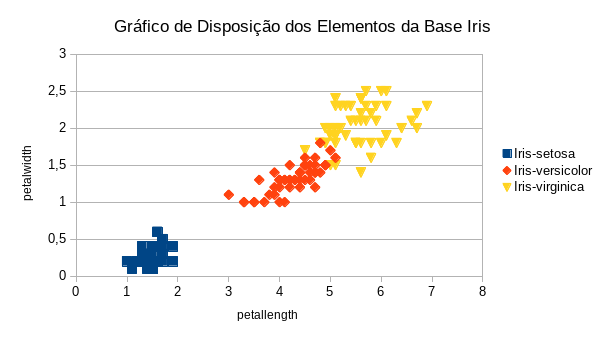
\includegraphics[scale=0.9]{figs/grafico_iris_petalwidth_petallength_BrOf.png}
        \caption{Gráfico da disposição de elementos da Base Iris entre os eixos \textbf{petallength} e \textbf{petalwidth}} \label{fig:grafico_iris_petalwidth_petallength_BrOf}
\end{figure}

Todos os algoritmos: Naive Bayes, CART e KNN, encontraram os mesmos rótulos em todos os \textit{clusters} da Iris, e ao analisar o gráfico, o \textit{cluster} 1 (Iris-setosa), é possível perceber uma relação bem definida entre os demais grupos, pois todos os elementos que possuem largura da pétala (\textit{petalwidth}) variando de 0.1 até 0.9 participam do grupo Iris-setosa, portanto, esse rótulo comprovadamente representa este grupo. Analisando os outros grupos através do gráfico da figura \ref{fig:grafico_iris_petalwidth_petallength_BrOf} percebe-se que a amostra de dados dos grupos Iris-versicolor e Iris-virginica contêm elementos que se misturam, não deixando um ponto de corte tão preciso quanto o da Iris-setosa, e isso acaba por também ocasionar ao rótulo alguns erros identificados nos \textit{clusters} 1 e 2.



\section{Base de Dados 3 - Glass - Identificação de Tipos de Vidros}\label{cap:resultados:ssec:iris}

Essa base ficou conhecida pelo Dr. Vina Spiehler, Ph.D. da DABFT Diagnostic Products Corporation, que conduziu pesquisas e testes de comparação em seu sistema baseado em regras, determinando se o tipo de vidro era temperado ou não. Institutos de investigação criminológica motivaram os estudos de classificação de tipos de vidro, porque em uma cena de crime, uma classificação de tipos de vidro corretamente identificada pode ser utilizada como prova, ajudando diretamente na investigação \cite{Evett:1989}.

Possui um total de 214 instancias, caracterizados por 9 atributos: índice de refração (RI), e os demais atributos correspondentes a porcentagem do óxido no Sódio (Na), Magnésio (Mg), Alumínio (Al), Silício (Si), Potássio (K), Cálcio (Ca), Bário (Ba) e Ferro (Fe).

Os tipos de vidro (atributo classe) foram divididos em 7 grupos distintos:
\begin{itemize} [noitemsep]
 \item janelas de construção - vidro temperado: 70 registros
 \item janelas de construção - vidro não-temperado: 76 registros
 \item janelas de veículos - vidro temperado: 17 registros
 \item janelas de veículos - vidro não-temperado: 0 registro
 \item recipientes: 13 registros
 \item louças de mesa: 9 registros
 \item lâmpadas: 29 registros 
\end{itemize}


Essa é uma base de dados diferente das demais por possuir mais grupos e, especificamente, o grupo de janelas de veículos - vidro não-temperado, que não possuem amostras de dados para exemplificar. Nos resultados dos rótulos exibidos nas tabelas adiante a coluna \textbf{Cluster}, que exibe uma sequência numérica dos grupos, não contemplará o grupo janelas de veículos - vidro não-temperado, pois não há exemplos de dados para definir o grupo, ficando somente seis grupos determinados na seguinte sequência : (1) janelas de construção - vidro temperado, (2) janelas de construção - vidro não-temperado, (3) janelas de veículos - vidro temperado, (4) recipientes , (5) louças de mesa e (6) lâmpadas. 

Nos teste desenvolvidos nesta pesquisa os valores de referência foram ${R=4}$ para o número de faixas, o método de discretização  e também a variância ${V}$ sofrerão alterações nas execuções nos próprios algoritmos para melhorar seus resultados. O que mais diferenciou os resultados desta base, foi ter que utilizar valores de ${V}$ bastantes altos para poder conseguir criar rótulos distintos.


\subsection{Naive Bayes} \label{cap:resultados:ssec:glass:nb}
%Os resultados da tabela \ref{tab:execucoes:glass:nb}, assim como nos resultados de bases anteriores, indicam uma sequência de execuções onde é possível observar o comportamento das variáveis que são escolhidas como rótulo. Nestes exemplos fica claro que não foi necessária a utilização de uma variação ${V}$ para a escolha dos rótulos, logo porque não houve ambiguidade entre eles. Por outro lado, quando testes utilizaram o outro método de discretização, EFD, retornaram rótulos ambíguos obrigando o uso da variação ${V}$. Em consequencia disto foi definindo o método de discretização EWD como padrão para a rotulação de dados.

Na aplicação desse algoritmo as melhores configurações para rotulação foram através do método EWD de discretização e a variação ${V=77\%}$ que influencia diretamente nas escolhas dos atributos. Esse valor foi necessário pois os resultados da matriz de importância apresentaram vários \textit{cluster} com rótulos iguais, desta forma foi realizado testes para chegar a um valor de ${V}$ para não haver mais ambiguidade.


A melhor maneira para explicar o valor de variância  ${V=77\%}$ é verificar na tabela \ref{tab:execucoes:glass:nb} (matriz de atributos importantes) os valores correspondentes aos \textit{clusters} que possuem rótulos iguais. Esta tabela contém os valores em porcentagem do quanto cada atributo é bem correlacionado com os demais, logo, quanto maior for o valor mais bem correlacionado é o atributo. Cada linha da tabela corresponde a um cluster e as colunas os atributos.



\begin{table}[!h]
\centering
\caption{Matriz de Atributos Importantes do algoritmo Naive Bayes na base Glass}
\label{tab:execucoes:glass:nb}
\scalebox{0.7}{

   %\small\addtolength{\tabcolsep}{-2pt} 
    \begin{tabular}{|cl|c|c|c|c|c|c|c|c|c|}
        \hline \hline
            {\tiny }     &   & \multicolumn{9}{c|}{\tiny Atributos}                                               \\ \cline{3-11} 
       \multicolumn{1}{|l}{}    &   & RI    & Na    & Mg  & Al   & Si   & K   & Ca   & Ba  & Fe             \\ \hline
        \multicolumn{1}{|c|}{}  & 1 & 8.5714 & 7.1429  & 4.2857 & 4.2857 & 8.5714 & 10.0 & 0 & 91.4286 & 58.5714 \\ \cline{2-11} 
        \multicolumn{1}{|c|}{}  & 2 & 2.6316  &  3.9474  &  14.4737  &  3.9474  &  0  & 11.8421  & 2.6316 & 85.5263  &  51.3158   \\ \cline{2-11} 
        \multicolumn{1}{|c|}{}  & 3 &  11.7647  &  17.6471  & 11.7647  &  0  &  0  & 5.8824  &  11.7647 & 94.1176  &  70.5882   \\ \cline{2-11}
        \multicolumn{1}{|c|}{}  & 4 &  0  &  0  &  46.1538  &  15.3846  &  0  &  15.3846  &  0  &  84.6154  &  84.6154  \\ \cline{2-11}
        \multicolumn{1}{|c|}{}  & 5 &  0  &  0  &  11.1111  &  0  &  0   & 100.00 &  0  &  100.00 & 100.00  \\ \cline{2-11}
        \multicolumn{1}{|c|}{\multirow{-3}{*}{\tiny Clusters}} & 6 &  6.8966  &  0  &  68.9655  &  6.8966  &  10.3448  &  48.2759  &  0  &  10.3448  & 58.6207  \\ \hline
        
        
    \end{tabular}

}
\end{table}    


O número da variância não é escolhido aleatoriamente, ao em vez disso, é analisada a matriz de atributos importantes, tabela  \ref{tab:execucoes:glass:nb}, e calculado o menor valor ${V}$ que contribua de forma a adicionar o menor número possíveis de atributos nos rótulos para  evitar a ambiguidade. Analisando esta tabela o valor encontrado ${V=77\%}$, foi o que obteve a distinção dos rótulos nos clusters, como também, fez com que um rótulo fosse contemplado com todos os atributos conforme pode-se conferir na tabela \ref{tab:rot:glass:nb}, que apresenta os seis clusters nas ordens sequenciais:(1) janelas de construção - vidro temperado, (2) janelas de construção - vidro não-temperado, (3) janelas de veículos - vidro temperado, (4) recipientes , (5) louças de mesa e (6) lâmpadas. 

\newpage
\begin{table}[!h]
\centering
\caption{Resultado da aplicação do algoritmo Naive Bayes}
\label{tab:rot:glass:nb}
\scalebox{0.8}{
\begin{tabular}{llcrcc} 
\hline \hline
 
\multicolumn{1}{c}{\cellcolor[HTML]{FFFFFF}} & \multicolumn{2}{c}{Rótulos}                & \multicolumn{1}{r}{}               & \\ \cline{2-3}
Cluster                                      & Atributos      & \multicolumn{1}{c}{Faixa} & \multicolumn{1}{c}{Relevância(\%)} & Fora da Faixa & Acurácia Parcial(\%)\\ \hline \hline
                                             & Ba     & [ 0.0 $\sim$  0.7875 ]   & 91\%  & 0 & 100\% \\  
\multirow{-2}{*}{1}                          & Fe    & [ 0.0 $\sim$  0.1275  ]   & 58\%  & 15 & 78.6\% \\  \hline
                                             & Mg    & ] 3.3675 $\sim$  4.49 ]   & 14\%  & 25 & 68\%\\ 
                                             & K     & [ 0.0 $\sim$  1.5525 ]     & 11\%  & 0  & 100\% \\  
                                            & Ba     & [ 0.0 $\sim$  0.7875 ]    & 85\%  & 1  & 98.7\% \\  
\multirow{-4}{*}{2}                          & Fe    & [ 0.0 $\sim$  0.1275 ]    & 51\%  & 23 & 69.8\% \\  \hline
                                            & Na     & ]12.3925 $\sim$  14.055 ] & 17\%  & 3  & 82.4\% \\ 
                                            & Ba     & [ 0.0 $\sim$  0.7875 ]    & 94\%  & 0  & 100\% \\  
\multirow{-3}{*}{3}                          & Fe    & [ 0.0 $\sim$  0.1275 ]    & 70\%  & 3  & 82.4\% \\  \hline
                                             & Mg    & [ 0.0 $\sim$  1.1225 ]    & 46\%  & 5  & 61.6\%\\ 
                                             & Al    & ] 1.0925 $\sim$  1.895]      & 15\%  & 4  & 69.3\%\\
                                            & K     & [  0.0 $\sim$  1.5525 ]    & 15\%  & 3  & 77\% \\ 
                                            & Ba     & [ 0.0 $\sim$  0.7875 ]    & 84\%  & 1  & 92.4\% \\  
\multirow{-5}{*}{4}                          & Fe    & [ 0.0 $\sim$  0.1275 ]    & 84\%  & 2  & 84.7\% \\  \hline                                            
                                            & K     & [ 0.00 $\sim$ 1.5525 ]     & 100\%  & 0 & 100\% \\ 
                                            & Ba     & [ 0.0 $\sim$  0.7875 ]    & 100\%  & 0 & 100\% \\  
\multirow{-3}{*}{5}                         & Fe    & [ 0.0 $\sim$  0.1275 ]     & 100\%  & 0 & 100\% \\  \hline
                                            & RI     & [1.511150 $\sim$  1.516845 ] & 6\%  & 11  & 62.1\% \\ 
                                            & Na     & ]14.055 $\sim$  15.7175 ] & 0\%  & 6  & 79.4\% \\ 
                                             & Mg    & [ 0.0 $\sim$  1.1225 ]    & 68\%  &6  & 79.4\%\\ 
                                             & Al    & ] 1.895 $\sim$  2.6975]      & 6\%  & 11  & 62.1\%\\
                                            & Si    & ] 72.61 $\sim$  74.01]      & 10\%  & 6  & 79.4\%\\
                                            & K     & [  0.0 $\sim$  1.5525 ]    & 15\%  & 2  & 93.2\% \\ 
                                            & Ca     & [ 8.12 $\sim$ 10.81 ]    & 0\%  & 3  & 89.7\% \\ 
                                            & Ba     & [ 0.0 $\sim$  0.7875 ]    & 10\%  & 15  & 48.3\% \\  
\multirow{-3}{*}{6}                         & Fe    & [ 0.0 $\sim$  0.1275 ]     & 58\%  & 0  & 100\% \\  \hline

\end{tabular}
}
\end{table}

Em análise dos resultados da execução do Naive Bayes os atributos \textbf{Ba} e \textbf{Fe} são os que aparecem em todos os rótulos indicando uma importância desses elementos nos grupos, que pode também ser percebido através dos altos valores de correlacionamento na tabela \ref{tab:execucoes:glass:nb}. Neste resultado observa-se que o cluster 6 acabou por ter um rótulo o qual todos os atributos estão selecionados, ou seja, fazem parte do rótulo, esse efeito foi causa da variância ${V}$ que atingiu um número maior, em relação ao resultado da diferença entre, o maior e menor valor  da linha respectiva a do cluster 6 da tabela \ref{tab:execucoes:glass:nb}. Dito isto, a variável cumpre seu papel de não deixar que rótulos repetidos existam.
% acurácia media p/ grupo
% cluster1=89.3
% cluster2=84.125
% cluster3=88.2
% cluster4=77
% cluster5 = 100
% cluster6=77.066

A menor acurácia média por grupo foi do cluster 4 (recipientes) com 77\%, e a maior acurácia do cluster 5 (louças de mesa) com 100\%.

De acordo com a aplicação do Naive Bayes na base de dados \textbf{Glass} os rótulos são os seguintes:
\begin{itemize}[noitemsep]
 \item ${r_{c_1}=\{ (Ba,[ 0.0 \sim 0.7875 ] ),(Fe,[ 0.0 \sim 0.1275 ] ) \} }$  
 \item ${r_{c_2}=\{ (Mg,] 3.3675 \sim  4.49 ] ),(K,[ 0.0 \sim 1.5525 ] ),(Ba,[ 0.0 \sim 0.7875 ] ),}$
 
 ${(Fe,[ 0.0 \sim 0.1275 ] ) \} }$
 \item ${r_{c_3}=\{ ((Na,]12.3925 \sim 14.055 ] ),(Ba,[ 0.0 \sim 0.7875 ] ),(Fe,[ 0.0 \sim 0.1275 ] )  \} }$  
 \item ${r_{c_4}=\{ (Mg,[ 0.0 \sim  1.1225 ] ),(Al,] 1.0925 \sim 1.895 ] ), (K,[ 0.0 \sim 1.5525 ] ),}$

 ${ (Ba,[ 0.0 \sim 0.7875 ] ),(Fe,[ 0.0 \sim 0.1275 ] ) \} }$
 \item ${r_{c_5}=\{  (K,[ 0.0 \sim 1.5525 ]  ),(Ba,[ 0.0 \sim 0.7875 ] ), (Fe,[ 0.0 \sim 0.1275 ] )\} }$
 \item ${r_{c_6}=\{ (RI,[ 1.511150 \sim  1.516845  ] ),(Na,]14.055 \sim 15.7175 ] ),  (Mg,[ 0.0 \sim  1.1225  ] ), }$
 
 ${ (Al,] 1.895 \sim 2.6975 ] ), (Si,] 72.61 \sim 74.01 ] ),  }$
 
 ${ (K,[ 0.0 \sim 1.5525] ),(Fe,[ 0.0 \sim 0.1275 ] ) \} }$
\end{itemize}


\subsection{Classification and Regression Trees - CART} \label{cap:resultados:ssec:glass:cart}

%Na execução do CART foi aplicado o método de discretização EWD e uma mudança no valor da variância ${V=6\%}$ para evitar a ambiguidade dos clusters 1 e 3. 

Através de testes foi descartado a utilização do método de discretização EFD, e adotado o EWD, em virtude da diminuirção de erros por atributo em comparação ao outro método, e a divisão de faixas foi mantido ${R=4}$. Quanto a variável ${V}$ sofreu alteração em relação ao algoritmo anterior, mas mesmo assim manteve-se alto com ${V=71\%}$, em razão do número de clusters com rótulos iguais. Este aumento da variável ${V}$ influencia diretamente, diminuindo a acurácia média do cluster, muito embora seja justificado esse aumento de ${V}$ devido os rótulos não poderem se repetir nos \textit{clusters}.

A execução do CART obteve os resultados apresentados na tabela \ref{tab:rot:glass:cart}.

\begin{table}[!h]
\centering
\caption{Resultado da aplicação do algoritmo CART}
\label{tab:rot:glass:cart}
\scalebox{0.8}{
\begin{tabular}{llcrcc} 
\hline \hline
 
\multicolumn{1}{c}{\cellcolor[HTML]{FFFFFF}} & \multicolumn{2}{c}{Rótulos}                & \multicolumn{1}{r}{}               & \\ \cline{2-3}
Cluster                                      & Atributos      & \multicolumn{1}{c}{Faixa} & \multicolumn{1}{c}{Relevância(\%)} & Fora da Faixa & Acurácia Parcial(\%)\\ \hline \hline
                                             & Ba     & [ 0.0 $\sim$  0.7875 ]   & 95\%  & 0 & 100\% \\  
\multirow{-2}{*}{1}                          & Fe    & [ 0.0 $\sim$  0.1275  ]   & 51\%  & 15 & 78.6\% \\  \hline
                                             & Mg    & ] 3.3675 $\sim$  4.49 ]   & 17\%  & 25 & 68\%\\ 
                                            & Ba     & [ 0.0 $\sim$  0.7875 ]    & 84\%  & 1  & 98.7\% \\  
\multirow{-3}{*}{2}                          & Fe    & [ 0.0 $\sim$  0.1275 ]    & 43\%  & 23 & 69.8\% \\  \hline
                                            & K     & [ 0.0 $\sim$  1.5525 ]     & 23\%  & 0  & 100\% \\ 
                                            & Ba     & [ 0.0 $\sim$  0.7875 ]    & 88\%  & 0  & 100\% \\  
\multirow{-3}{*}{3}                          & Fe    & [ 0.0 $\sim$  0.1275 ]    & 70\%  & 3  & 82.7\% \\  \hline
                                             & Mg    & [ 0.0 $\sim$  1.1225 ]    & 30\%  & 5  & 61.6\%\\ 
                                             & Al    & ] 1.43 $\sim$  1.83]      & 15\%  & 4  & 69.3\%\\
                                            & K     & [  0.0 $\sim$  1.5525 ]    & 15\%  & 3  & 77\% \\ 
                                            & Ba     & [ 0.0 $\sim$  0.7875 ]    & 76\%  & 1  & 92.4\% \\  
\multirow{-5}{*}{4}                          & Fe    & [ 0.0 $\sim$  0.1275 ]    & 69\%  & 2  & 84.7\% \\  \hline
                                            & Mg    & [ 0.0 $\sim$  1.1225 ]     & 33\%  & 5  & 44.5\% \\ 
                                            & K     & [ 0.00 $\sim$ 1.5525 ]     & 100\%  & 0 & 100\% \\ 
                                            & Ba     & [ 0.0 $\sim$  0.7875 ]    & 100\%  & 0 & 100\% \\  
\multirow{-4}{*}{5}                         & Fe    & [ 0.0 $\sim$  0.1275 ]     & 100\%  & 0 & 100\% \\  \hline
                                            & Mg    & [ 0.0 $\sim$  1.1225 ]     & 65\%  & 6  & 79.4\% \\ 
                                            & K     & [ 0.0 $\sim$ 1.5525 ]      & 48\%  & 2  & 93.2\% \\ 
\multirow{-3}{*}{6}                         & Fe    & [ 0.0 $\sim$  0.1275 ]     & 79\%  & 0  & 100\% \\  \hline

\end{tabular}
}
\end{table}

As acurácias parciais foram bem diversificadas bem como o número de atributos por rótulo, embora mais uma vez os elementos \textbf{Ba} e \textbf{Fe} são os atributos que aparecem com mais frequência mantendo os mesmos intervalos de dados. Fazendo um cálculo da acurácia média por grupo, os valores variam de 77\% o menor valor no grupo \textit{recipientes}, e 90.8\% o maior valor no grupo \textit{lâmpadas}, apesar de saber que esses valores poderiam melhorar caso não tivessem tantos rótulos atribuído pela variável ${V}$ é a forma de manter um rótulo único por grupo.
% acurácia media p/ grupo
% cluster1=89.3
% cluster2=78.8
% cluster3=94.2
% cluster4=77
% cluster5 = 86.1
% cluster6=90.8



De acordo com a aplicação do CART na base de dados \textbf{Glass} os rótulos são os seguintes:
\begin{itemize}[noitemsep]
 \item ${r_{c_1}=\{ (Ba,[ 0.0 \sim 0.7875 ] ),(Fe,[ 0.0 \sim 0.1275 ] ) \} }$  
 \item ${r_{c_2}=\{ (Mg,] 3.3675 \sim  4.49 ] ),(Ba,[ 0.0 \sim 0.7875 ] ),(Fe,[ 0.0 \sim 0.1275 ] ) \} }$
 \item ${r_{c_3}=\{ ((K,[ 0.0 \sim 1.5525 ] ),(Ba,[ 0.0 \sim 0.7875 ] ),(Fe,[ 0.0 \sim 0.1275 ] )  \} }$  
 \item ${r_{c_4}=\{ (Mg,[ 0.0 \sim  1.1225 ] ),(Al,] 1.0925 \sim 1.895 ] ), (K,[ 0.0 \sim 1.5525 ] ),}$

 ${ (Ba,[ 0.0 \sim 0.7875 ] ),(Fe,[ 0.0 \sim 0.1275 ] ) \} }$
 \item ${r_{c_5}=\{ (Mg,[ 0.0 \sim  1.1225 ] ), (K,[ 0.0 \sim 1.5525 ]  ),(Ba,[ 0.0 \sim 0.7875 ] ), }$
 
 ${ (Fe,[ 0.0 \sim 0.1275 ] ) \} }$
 \item ${r_{c_6}=\{ (Mg,[ 0.0 \sim  1.1225  ] ),  (K,[ 0.0 \sim 1.5525] ),(Fe,[ 0.0 \sim 0.1275 ] ) \} }$
\end{itemize}



\subsection{K-Nearest Neighbor - KNN} \label{cap:resultados:ssec:glass:knn}


Na tabela \ref{tab:rot:glass:knn} é apresentado o resultado da execução do algoritmo KNN na base de dados Glass aplicando o método de discretização EWD, com valor da variância ${V=81\%}$ e alterando para ${R=3}$. Na mesma situação do Naive Bayes, o cluster 6 recebeu um rótulo com todos os atributos, pelo alto valor de ${V}$, embora necessário para retirar as ambiguidades dos rótulos a consequência é aumentar o números de atributos nos rótulos, implicando também na diminuição da acurácia média por grupo. 

\newpage
\begin{table}[!h]
\centering
\caption{Resultado da aplicação do algoritmo KNN}
\label{tab:rot:glass:knn}
\scalebox{0.8}{
\begin{tabular}{llcrcc} 
\hline \hline
 
\multicolumn{1}{c}{\cellcolor[HTML]{FFFFFF}} & \multicolumn{2}{c}{Rótulos}                & \multicolumn{1}{r}{}               & \\ \cline{2-3}
Cluster                                      & Atributos      & \multicolumn{1}{c}{Faixa} & \multicolumn{1}{c}{Relevância(\%)} & Fora da Faixa & Acurácia Parcial(\%)\\ \hline \hline
                                             & Al   & [ 0.29 $\sim$  1.36 ]     & 15\%  & 10  & 85.8\% \\  
                                            & K     & [ 0.0 $\sim$  2.07 ]     & 24\%  & 0  & 100\% \\  
                                             & Ba    & [ 0.0 $\sim$  1.05 ]   & 95\%  & 0 & 100\% \\  
\multirow{-4}{*}{1}                          & Fe    & [ 0.0 $\sim$  0.17  ]   & 64\%  & 8 & 88.6\% \\  \hline
                                             & Mg    & ] 2.993333 $\sim$  4.49 ]   & 18\%  & 19 & 75\%\\ 
                                             & K     & [ 0.0 $\sim$  2.07 ]     & 18\%  & 0  & 100\% \\
                                            & Ba     & [ 0.0 $\sim$ 1.05 ]    & 92\%  & 1  & 98.7\% \\  
\multirow{-4}{*}{2}                          & Fe    & [ 0.0 $\sim$  0.17 ]    & 51\%  & 16 & 79\% \\  \hline
                                            & Ba     & [ 0.0 $\sim$  1.05 ]    & 94\%  & 0  & 100\% \\  
\multirow{-2}{*}{3}                          & Fe    & [ 0.0 $\sim$   0.17 ]    & 70\%  & 2  & 88.3\% \\  \hline
                                             & Mg    & [ 0.0 $\sim$  1.496667 ]    & 53\%  & 5  & 61.6\%\\ 
                                             & Al    & ] 1.36 $\sim$  2.43]      & 15\%  & 3  & 77\%\\
                                            & K     & [  0.0 $\sim$  2.07 ]    & 15\%  & 2  & 84.7\% \\ 
                                            & Ba     & [ 0.0 $\sim$  1.05 ]    & 84\%  & 1  & 92.4\% \\  
\multirow{-5}{*}{4}                          & Fe    & [ 0.0 $\sim$  0.17 ]    & 84\%  & 2  & 84.7\% \\  \hline                                            
                                            & K     & [ 0.00 $\sim$  2.07 ]     & 100\%  & 0 & 100\% \\ 
                                            & Ba     & [ 0.0 $\sim$  1.05 ]    & 100\%  & 0 & 100\% \\  
\multirow{-3}{*}{5}                         & Fe    & [ 0.0 $\sim$  0.17 ]     & 100\%  & 0 & 100\% \\  \hline
                                            & RI     & [1.511150 $\sim$  1.516845 ] & 0\%  & 4  & 86.3\% \\ 
                                            & Na     & ]12.946667 $\sim$  15.163333 ] & 3\%  & 2  & 93.2\% \\ 
                                             & Mg    & [ 0.0 $\sim$  1.1225 ]    & 79\%  &6  & 79.4\%\\ 
                                             & Al    & [ 0.0 $\sim$  1.496667]      & 6\%  & 10  & 65.6\%\\
                                            & Si    & ] 71.676667 $\sim$  73.543333]      & 6\%  & 6  & 79.4\%\\
                                            & K     & [  0.0 $\sim$  2.07 ]    & 55\%  & 1  & 96.6\% \\ 
                                            & Ca     & [5.43 $\sim$ 9.016667 ]    & 3\%  & 7  & 75.9\% \\ 
                                            & Ba     & [ 0.0 $\sim$ 1.05 ]    & 20\%  & 14  & 51.8\% \\ 
\multirow{-9}{*}{6}                         & Fe    & [ 0.0 $\sim$  0.17 ]     & 75\%  & 0  & 100\% \\  \hline\hline

\end{tabular}
}
\end{table}
% cluster 1=93,6
% cluster 2=88,175
% cluster 3=94,15
% cluster 4=80,08
% cluster 5=100
% cluster 6=80,9111111111111

Analisando os resultados percebe-se que a acurácia média por rótulo foi acima dos 80\% indicando que cada tipo de vidro  é representado de forma satisfatória pelos rótulos dos grupos. As valores nos elementos químicos (atributos) é uma porcentagem de óxido que varia de acordo com o vidro, e  com essas informações é possível identicar o tipo de vidro, \textit{i.e.}, para identificar um tipo de vidro olhando para os elementos químicos Mg, K, Ba e Fe, que são atributos do ${r_{c_2}}$, basta verificar os valore de óxido em cada um desses elementos, e se as informações forem compatíveis, então ele é do tipo, janela de construção - vidro não-temperado. Mesmo que os elementos estejam se repetindo no ${r_{c_6}}$, a faixa de valor do elemento químico Mg é diferente entre os rótulos, garantindo que os rótulos consigam representar cada grupo. 
%A acurácia média por grupo varia da menor de 80\% até 100\% referente ao cluster 5. 


De acordo com a aplicação do KNN na base de dados \textbf{Glass} os rótulos são os seguintes:
\begin{itemize}[noitemsep]
 \item ${r_{c_1}=\{(Al,[ 0.29 \sim 1.36 ] ),(K,[ 0.0 \sim  2.0700 ] ), (Ba,[ 0.0 \sim 1.05 ] ),}$
 
 ${ (Fe,[ 0.0 \sim 0.17] )  \} }$
 \item ${r_{c_2}=\{(Mg, [ 2.993333 \sim  4.490]),(K,[ 0.0 \sim  2.0700 ] ), (Ba,[ 0.0 \sim 1.05 ] ),}$
 
 ${ (Fe,[ 0.0 \sim 0.17] )  \} }$
 \item ${r_{c_3}=\{ (Ba,[ 0.0 \sim 1.0500 ] ),(Fe,[ 0.0 \sim 0.17] )  \} }$
 \item ${r_{c_4}=\{(Mg, [ 2.993333 \sim  4.490]), (Al,[ 0.29 \sim 1.36 ] ),(K,[ 0.0 \sim  2.0700 ] ),}$
 
 ${ (Ba,[ 0.0 \sim 1.0500 ] ), (Fe,[ 0.0 \sim 0.17] )  \} }$
 \item ${r_{c_5}=\{ (K,[ 0.0 \sim  2.0700 ] ), (Ba,[ 0.0 \sim 1.0500 ] ), (Fe,[ 0.0 \sim 0.17000] ) \} }$
 \item ${r_{c_6}=\{ (RI,[ 1.511150 \sim  1.516845  ] ),(Na,]12.946667 \sim 15.163333 ] ),  (Mg,[ 0.0 \sim  1.1225  ] ), }$
 
 ${ (Al,[0.0 \sim  1.496667 ] ), (Si,] 71.676667 \sim  73.543333 ] ),  }$
 
 ${ (K,[ 0.0 \sim 2.07] ),(Fe,[ 0.0 \sim 0.17 ] ) \} }$
\end{itemize}


\subsection{Comparativo entre Algoritmos na Base de Dados Glass} \label{cap:resultados:ssec:compalgoritmos:glass}

Diferentes das outras bases testadas o método de discretização EWD, na base Glass, fez com que os resultados dos rótulos fossem melhores, pois não houve tantas repetições de rótulos entre os \textit{clusters} implicando em uma acurácia parcial mais alta. Um exemplo do rótulo na base Glass utilizando KNN com método de discretização EFD está a seguir:
\begin{itemize}[noitemsep]
 \item ${r_{c_1}=\{ (Ba,[ 0.0 \sim 0.54 ] )\} }$
 \item ${r_{c_2}=\{(Ba,[ 0.0 \sim 0.54 ] ) \} }$
 \item ${r_{c_3}=\{ (Ba,[ 0.0 \sim 0.54 ])  \} }$  
 \item ${r_{c_4}=\{ (Mg,[ 0.0 \sim 3.09 ] ) \}}$
 \item ${r_{c_5}=\{ (Na,[13.75 \sim  17.38 ] ), (Mg,[ 0.0 \sim 3.09 ] ), }$
 
 ${(K,[ 0.0 \sim 0.31 ] ), (Ba,[ 0.0 \sim 0.54 ] ), (Fe,[ 0.0 \sim 0.11] ) \} }$
 \item ${r_{c_6}=\{ (Fe,[ 0.0 \sim 0.11] ) \} }$
\end{itemize}

Pode-se notar deste resultado acima, que os \textit{clusters} 1, 2 e 3 já apresentavam problemas, por possuírem rótulos iguais, e para contornar essa situação teria que inserir valores na variância ${V}$ a fim de tirar essas ambiguidades, mas isso, gera um aumento no número de atributos rótulos, e por consequência, também pode diminuir as  acurácias parciais, portanto, para alterar este resultado do rótulo, foi utilizado EWD, como método de discretização da bases de dados.
 
Em relação aos resultados apresentados entre os três algoritmos o KNN teve as melhores acurácias parciais, pois mesmo com semelhanças entre os rótulos, pode-se dizer que o KNN pegou o melhor dos dois rótulos, Naive Bayes e CART, e ficando com os rótulos que tiveram menores erros, por consequência, melhores acurácias parciais, e para verificar esta afirmativa, pode-se comparar os resultados \textit{cluster} por \textit{cluster} a partir da tabela \ref{tab:comparativo:bases}.

\begin{table}[!h]
\caption{Resultado comparativo \textit{cluster} por \textit{cluster} entre Naive Bayes (NB), CART e KNN. }

   % \hspace{1cm} %altera o espaçamento entre as tabelas
   \subfloat[Cluster 1 - janelas de construção - vidro temperado ]{ \label{tab:comparativo:bases:cluster1}
   \scalebox{0.8}{
   \small\addtolength{\tabcolsep}{-2pt} 
    \begin{tabular}{|l|l|l|l|l|l|}
        \hline
        \multicolumn{2}{|c|}{NB} & \multicolumn{2}{c|}{CART} & \multicolumn{2}{c|}{KNN} \\ \hline
          Atrib  & Acur(\%) & Atrib  & Acur(\%)  & Atrib  & Acur(\%) \\ \hline
            &        &   Mg      & 94        &           &              \\ \hline
            &        &     Si    & 94        &           &              \\ \hline
            K & 100   &   K       & 100       &   K       & 100          \\ \hline
            Ba & 100  &    Ba     & 100       &    Ba     & 100            \\ \hline
    \end{tabular}
   }}
 %&
    \hspace{1cm} %altera o espaçamento entre as tabelas
   \subfloat[Cluster 2 - janelas de construção - vidro não-temperado]{ \label{tab:comparativo:bases:cluster2}
   \scalebox{0.8}{
   \small\addtolength{\tabcolsep}{-2pt}
   \begin{tabular}{|l|l|l|l|l|l|}
      \hline 
      \multicolumn{2}{|c|}{NB} & \multicolumn{2}{c|}{CART} & \multicolumn{2}{c|}{KNN} \\ \hline
        Atrib  & Acur(\%) & Atrib  & Acur(\%)  & Atrib  & Acur(\%) \\ \hline
             K & 100           &       K & 100            &       K & 100          \\ \hline
               &              &      Ba & 98             &           &              \\ \hline
   \end{tabular}
  }}
     
    \subfloat[Cluster 3 - janelas de veículos - vidro temperado]{ \label{tab:comparativo:bases:cluster3}
    \scalebox{0.8}{
    \small\addtolength{\tabcolsep}{-2pt} 
    \begin{tabular}{|l|l|l|l|l|l|}
        \hline
        \multicolumn{2}{|c|}{NB} & \multicolumn{2}{c|}{CART} & \multicolumn{2}{c|}{KNN} \\ \hline
            Atrib  & Acur(\%) & Atrib  & Acur(\%)  & Atrib  & Acur(\%) \\ \hline
               Mg  & 100      &   Mg   & 100       &   Mg   & 100         \\ \hline
                 K & 100   &   K       & 100       &   K    & 100          \\ \hline
                Ba & 100  &    Ba     & 100       &    Ba  & 100            \\ \hline
    \end{tabular}
    }}
%     %&
    \hspace{1cm}
    \subfloat[Cluster 4 - recipientes]{  \label{tab:comparativo:bases:cluster4}
    \scalebox{0.8}{
    \small\addtolength{\tabcolsep}{-2pt}
    \begin{tabular}{|l|l|l|l|l|l|}
    \hline
    \multicolumn{2}{|c|}{NB} & \multicolumn{2}{c|}{CART} & \multicolumn{2}{c|}{KNN} \\ \hline
        Atrib  & Acur(\%) & Atrib  & Acur(\%)  & Atrib  & Acur(\%) \\ \hline
               &     &    RI  &   92      &           &              \\ \hline
        Al    &   92  &    Al  &   92      &           &              \\ \hline
         K     & 92    &       &         &           &              \\ \hline
        Ca     &  92   &   Ca   &  92       &           &              \\ \hline
        Ba     &    92 &    Ba  &    92     &     Ba     &    92      \\ \hline
    \end{tabular}
   %\\
    }}
    
    \subfloat[Cluster 5 - louças de mesa]{  \label{tab:comparativo:bases:cluster5}
    \scalebox{0.8}{
    \small\addtolength{\tabcolsep}{-2pt}
    \begin{tabular}{|l|l|l|l|l|l|}
    \hline
    \multicolumn{2}{|c|}{NB} & \multicolumn{2}{c|}{CART} & \multicolumn{2}{c|}{KNN} \\ \hline
        Atrib  & Acur(\%) & Atrib  & Acur(\%)  & Atrib  & Acur(\%) \\ \hline
         K     & 100     &   K       & 100    &   K    & 100          \\ \hline
            Ba & 100     &    Ba     & 100    &    Ba  & 100            \\ \hline
       Fe      & 100     & Fe        & 100    & Fe      & 100                   \\ \hline
    \end{tabular}
   }}
%         
   \hspace{1cm}    
   \subfloat[Cluster 6 - lâmpadas]{  \label{tab:comparativo:bases:cluster6}
   \scalebox{0.8}{
   \small\addtolength{\tabcolsep}{-2pt}
   \begin{tabular}{|l|l|l|l|l|l|}
    \hline
    \multicolumn{2}{|c|}{NB} & \multicolumn{2}{c|}{CART} & \multicolumn{2}{c|}{KNN} \\ \hline
        Atrib  & Acur(\%) & Atrib  & Acur(\%)  & Atrib  & Acur(\%) \\ \hline
               &              &      K     & 96        &           &              \\ \hline
        Fe     & 100         &       Fe     & 100       &      Fe     & 100        \\ \hline

\end{tabular}
   %\\
    }}

\label{tab:comparativo:bases}
\end{table}


De acordo com a tabela \ref{tab:comparativo:bases} é feito um comparativo entre os \textit{cluster} dos três algoritmos,  o Naive Bayes e CART e KNN, e percebe-se que o CART é o algoritmo que mais se diferencia entre os outros. Nos resultados de Naive Bayes e CART, os rótulos diferenciados são: \textit{cluster} 1 (tabela \ref{tab:comparativo:bases:cluster1}), 2 (tabela \ref{tab:comparativo:bases:cluster2}) e 6 (tabela \ref{tab:comparativo:bases:cluster6}). No  Naive Bayes e KNN, os rótulos são bem semelhantes, diferenciados somente pelo \textit{cluster} 4 (tabela \ref{tab:comparativo:bases:cluster4}), que como rótulo do KNN, possui apenas o atributo \textbf{Ba}, com intervalor de [0.0 até 1.05]. Já entre o CART e KNN possuem mais diferenças entre os \textit{clusters}, coincidindo somente nos \textit{clusters} 3 (tabela \ref{tab:comparativo:bases:cluster3}) e 6 (tabela \ref{tab:comparativo:bases:cluster6}). Percebe-se que o algoritmo CART foi o que encontrou rótulos mais diferentes entre os resultados dos outros dois algoritmos, mas isso se deve ao fato da utilização da variação ${V=6\%}$ que implicou no acréscimo de  atributos nos rótulos de alguns \textit{clusters}.

%mas isso se deve ao fato do método de discretização, EWD, utilizado no CART, deixando as faixas diferenciadas e implicando em rótulos também diferentes.


\section{Base de Dados 4 - Wine - Dados de Reconhecimento de vinhos}

Essa base \cite{Aeberhard1992} possui dados que são resultados de uma análise química de vinhos em uma mesma região da Itália, mas com três tipos de cultivos diferenciados, resultando em três classes distintas (tipos de vinho), e totalizando 178 registros. Através desta análise foi determinado treze características determinantes para classificação do tipo de vinho, que estão distribuídas em 178 amostras, e  esses treze atributos são: (1) álcool , (2) ácido málico - AM, (3) cinzas, (4) alcalinidade das cinzas - AC, (5) magnésio, (6) total de fenois - TF, (7) flavonoides, (8) fenóis não-flavonoides - FnF, (9) proantocianidinas, (10) intensidade da cor - IC, (11) matiz, (12) OD280/OD315 de vinhos diluídos - OD e (13) prolina.

A divisão em número de instâncias por classe são:

\begin{itemize}[noitemsep]
 \item classe 1: 59 elementos;
 \item classe 2: 71 elementos;
 \item classe 3: 48 elementos;
\end{itemize}

Na descrição da base Wine\footnote{https://archive.ics.uci.edu/ml/machine-learning-databases/wine/wine.names} não é dito qual seriam os nomes das classes (tipos de vinho), designados como classe 1, 2 ou 3, portanto, os rótulos encontrados pelos algoritmos são apresentados em tabelas, e na coluna \textbf{Cluster} as informações são inseridas por sequência numéria: \textit{cluster} 1, \textit{cluster} 2, \textit{cluster} 3 com 59, 71 e 48 registros respectivamente.

Na aplicação dos três algoritmos a seguir, foram  utilizados o método de discretização EWD, ao invés do EFD, pois obtiveram melhores resultados nos rótulos encontrados, e foi mantido o ${R=3}$ para todos os atributos, e também a variância ${V=0\%}$.

\subsection{Naive Bayes} \label{cap:resultados:ssec:wine:bayes}

Os rótulos encontrados após aplicação do Naive Bayes é apresentado na tabela \ref{tab:rot:wine:nb}, e separado por cluster 1, 2 e 3 representando os três tipos de vinho. Cada \textit{cluster} teve somente um atributo, e sua faixa respectiva, como rótulo.

\begin{table}[!h]
\centering
\caption{Resultado da aplicação do algoritmo Naive Bayes}
\label{tab:rot:wine:nb}
\scalebox{0.7}{
\begin{tabular}{llcrcc} 
\hline \hline
 
\multicolumn{1}{c}{\cellcolor[HTML]{FFFFFF}} & \multicolumn{2}{c}{Rótulos}                & \multicolumn{1}{r}{}               & \\ \cline{2-3}
Cluster                                      & Atributos      & \multicolumn{1}{c}{Faixa} & \multicolumn{1}{c}{Relevância(\%)} & Fora da Faixa & Acurácia Parcial(\%)\\ \hline \hline
 
1                                           & matiz     & ] 0.890000 $\sim$  1.3000  ]       & 91\%      & 7 & 91\% \\  \hline
2                                            & IC       & [ 1.28000 $\sim$  5.186667 ]           & 95\%  & 3 & 95\% \\  \hline
3                                         & flavonoides & [ 0.3400 $\sim$  1.9200 ]      & 100\%         & 0 &  100\% \\  \hline
\hline
\end{tabular}}
\end{table}


De acordo com a aplicação do Naive Bayes na base de dados \textbf{Wine} os rótulos são:

\begin{itemize}[noitemsep]
    \item ${r_{c_1}=\{ (matiz, ] 0.890000 \sim  1.3000])\} }$
    \item ${r_{c_2}=\{(IC,[  1.28000 \sim  5.186667  ] ) \} }$
    \item ${r_{c_3}=\{ (flavonoides, [ 0.3400 \sim  1.9200])\} }$
 \end{itemize}


\subsection{Classification and Regression Trees - CART} \label{cap:resultados:ssec:wine:cart}

Na tabela \ref{tab:rot:wine:cart} apresenta os rótulos encontrados pelo CART na base Wine, e pode-se perceber, através dos resultados, que o \textit{cluster} 3, foi o que melhor representou os rótulos, pois obteve uma acurácia de ${100\%}$, indicando que o vinho pertence ao terceiro grupo, e possui como característica principal o \textbf{flavonoides} variando no intervalo de 0.34 a 1.92. Para um especialista, ao reparar essa característica em um vinho, ele já saberia em qual grupo ele pertenceria, só utilizando esse conhecimento do rótulo.

\begin{table}[!h]
\centering
\caption{Resultado da aplicação do algoritmo CART}
\label{tab:rot:wine:cart}
\scalebox{0.8}{
\begin{tabular}{llcrcc} 
\hline \hline
 
\multicolumn{1}{c}{\cellcolor[HTML]{FFFFFF}} & \multicolumn{2}{c}{Rótulos}                & \multicolumn{1}{r}{}               & \\ \cline{2-3}
Cluster                                      & Atributos      & \multicolumn{1}{c}{Faixa} & \multicolumn{1}{c}{Relevância(\%)} & Fora da Faixa & Acurácia Parcial(\%)\\ \hline \hline
 
1                                           & matiz     & ] 0.890000 $\sim$  1.3000  ]       & 84\%      & 7 & 91\% \\  \hline
2                                            & IC       & [ 1.28000 $\sim$  5.186667 ]       & 94\%  & 3 & 95\% \\  \hline
3                                         & flavonoides & [ 0.3400 $\sim$  1.9200 ]      & 100\%         & 0 &  100\% \\  \hline
\hline
\end{tabular}}
\end{table}

Logo os rótulos da aplicação do CART na base de dados \textbf{Wine} são:
\begin{itemize}[noitemsep]
    \item ${r_{c_1}=\{ (matiz, ] 0.890000 \sim  1.3000])\} }$
    \item ${r_{c_2}=\{(IC,[  1.28000 \sim  5.186667  ] ) \} }$
    \item ${r_{c_3}=\{ (flavonoides, [ 0.3400 \sim  1.9200])\} }$
 \end{itemize}
 
 
\subsection{K-Nearest Neighbor - KNN} \label{cap:resultados:ssec:wine:knn}

No resultado do KNN, na tabela \ref{tab:rot:wine:knn},  atributo \textbf{flavonoides} se repete no \textit{cluster} 1, e \textit{cluster} 2, porém seus intervalos são diferentes, e isso garante a individualidade dos rótulos. Caso estas faixas fossem também iguais, teria que fazer o uso da variância ${V}$, mas que neste caso não é preciso. 

\begin{table}[!h]
\centering
\caption{Resultado da aplicação do algoritmo KNN}
\label{tab:rot:wine:knn}
\scalebox{0.8}{
\begin{tabular}{llcrcc} 
\hline \hline
 
\multicolumn{1}{c}{\cellcolor[HTML]{FFFFFF}} & \multicolumn{2}{c}{Rótulos}                & \multicolumn{1}{r}{}               & \\ \cline{2-3}
Cluster                                      & Atributos      & \multicolumn{1}{c}{Faixa} & \multicolumn{1}{c}{Relevância(\%)} & Fora da Faixa & Acurácia Parcial(\%)\\ \hline \hline
 
1                                           & flavonoides     & ] 1.920000 $\sim$  3.500000  ]       & 93\%      & 7 & 88\% \\  \hline
2                                            & IC       & [ 1.28000 $\sim$  5.186667 ]       & 95\%  & 3 & 95\% \\  \hline
3                                         & flavonoides & [ 0.3400 $\sim$  1.9200 ]      & 100\%         & 0 &  100\% \\  \hline
\hline
\end{tabular}}
\end{table}

Em uma analise, parecida, com aquela feita no CART, um especialista conhece através dos valores do flavonoides, qual o grupo do vinho ele pertence, pois se fizer parte da primeira faixa, é do \textit{cluster} 1, e caso o mesmo atributo, flavonoides, tiver um valor na faixa de ]0.34 a 1.92] é do \textit{cluster} 2.

Os rótulos encontrados  após a execução do KNN na base \textbf{Wine} são:
\begin{itemize}[noitemsep] 
    \item ${r_{c_1}=\{ (flavonoides, ] 1.920000 \sim  3.500000])\} }$
    \item ${r_{c_2}=\{(IC,[  1.28000 \sim  5.186667  ] ) \} }$
    \item ${r_{c_3}=\{ (flavonoides, [ 0.3400 \sim  1.9200])\} }$
 \end{itemize}



\subsection{Comparativo entre Algoritmos na Base de Dados Wine} \label{cap:resultados:ssec:compalgoritmos:wine}

Os resultados dos rótulos dos três algoritmos (Naive Bayes, CART e KNN), foram bastantes semelhantes, e em específico os dois, Naive Bayes e CART, são idênticos, havendo diferença no \textit{cluster} 1 do algoritmo KNN, em relação aos outros dois algoritmos.  

Nas tabelas \ref{tab:analise:wine:cluster1:matiz} e \ref{tab:analise:wine:cluster1:flavonoides} possuem uma amostra de registros do \textit{cluster} 1, onde é possível perceber quais os registros estão fazendo parte dos rótulos encontrados em cada algoritmo através das linhas em destaque. A tabela é formada pela primeira coluna indicando o número do registro na base de dados e em seguida os atributos.

\begin{table}[!ht]
\centering
\caption{Amostra do \textit{cluster} 1 da base dados Wine, ordenados pelo atributo \textbf{matiz}}
\label{tab:analise:wine:cluster1:matiz}
\scalebox{0.8}{
\small\addtolength{\tabcolsep}{-2pt}
\begin{tabular}{|c|c|c|c|c|c|c|c|c|c|c|c|c|c|}
\hline 
 n. & álcool & AM & cinza & AC & magnésio & TF & flavonoides & FnF & proantocianidinas & IC & matiz & OD & prolina \\ \hline
  
1 & 13,24 & 3,98 & 2,29 & 17,5 & 103 & 2,64 & 2,63 & 0,32 & 1,66 & 4,36 & 0,82 & 3 & 680\\ \hline
2 & 14,37 & 1,95 & 2,5 & 16,8 & 113 & 3,85 & 3,49 & 0,24 & 2,18 & 7,8 & 0,86 & 3,45 & 1480\\ \hline
3 & 14,21 & 4,04 & 2,44 & 18,9 & 111 & 2,85 & 2,65 & 0,3 & 1,25 & 5,24 & 0,87 & 3,33 & 1080\\ \hline
4 & 13,05 & 1,77 & 2,1 & 17 & 107 & 3 & 3 & 0,28 & 2,03 & 5,04 & 0,88 & 3,35 & 885\\ \hline
5 & 13,88 & 1,89 & 2,59 & 15 & 101 & 3,25 & 3,56 & 0,17 & 1,7 & 5,43 & 0,88 & 3,56 & 1095\\ \hline
6 & 14,22 & 3,99 & 2,51 & 13,2 & 128 & 3 & 3,04 & 0,2 & 2,08 & 5,1 & 0,89 & 3,53 & 760\\ \hline
7 & 13,72 & 1,43 & 2,5 & 16,7 & 108 & 3,4 & 3,67 & 0,19 & 2,04 & 6,8 & 0,89 & 2,87 & 1285\\ \hline
 \rowcolor[HTML]{EFEFEF} 
8 & 13,41 & 3,84 & 2,12 & 18,8 & 90 & 2,45 & 2,68 & 0,27 & 1,48 & 4,28 & 0,91 & 3 & 1035\\ \hline
 \rowcolor[HTML]{EFEFEF} 
9 & 13,9 & 1,68 & 2,12 & 16 & 101 & 3,1 & 3,39 & 0,21 & 2,14 & 6,1 & 0,91 & 3,33 & 985\\ \hline
... & ... & ... & ... & ... & ... & ... & ... & ... & ... & ... & ...& ... & ... \\ \hline
 \rowcolor[HTML]{EFEFEF} 
58 & 14,75 & 1,73 & 2,39 & 11,4 & 91 & 3,1 & 3,69 & 0,43 & 2,81 & 5,4 & 1,25 & 2,73 & 1150\\ \hline
 \rowcolor[HTML]{EFEFEF} 
59 & 13,63 & 1,81 & 2,7 & 17,2 & 112 & 2,85 & 2,91 & 0,3 & 1,46 & 7,3 & 1,28 & 2,88 & 1310\\ \hline
  \end{tabular}}
  \end{table}
  
  \begin{table}[!ht]
\centering
\caption{Amostra do \textit{cluster} 1 da base dados Wine, ordenados pelo atributo \textbf{flavonoides}}
\label{tab:analise:wine:cluster1:flavonoides}
  \scalebox{0.8}{
  \small\addtolength{\tabcolsep}{-2pt}
  \begin{tabular}{|c|c|c|c|c|c|c|c|c|c|c|c|c|c|}
   
\hline
n. & álcool & AM & cinza & AC & magnésio & TF & flavonoides & FnF & proantocianidinas & IC & matiz & OD & prolina \\ \hline
 \rowcolor[HTML]{EFEFEF} 
1 & 13,3 & 1,72 & 2,14 & 17 & 94 & 2,4 & 2,19 & 0,27 & 1,35 & 3,95 & 1,02 & 2,77 & 1285 \\ \hline
 \rowcolor[HTML]{EFEFEF} 
2 & 14,02 & 1,68 & 2,21 & 16 & 96 & 2,65 & 2,33 & 0,26 & 1,98 & 4,7 & 1,04 & 3,59 & 1035 \\ \hline
 \rowcolor[HTML]{EFEFEF} 
3 & 12,85 & 1,6 & 2,52 & 17,8 & 95 & 2,48 & 2,37 & 0,26 & 1,46 & 3,93 & 1,09 & 3,63 & 1015 \\ \hline
 \rowcolor[HTML]{EFEFEF} 
4 & 12,93 & 3,8 & 2,65 & 18,6 & 102 & 2,41 & 2,41 & 0,25 & 1,98 & 4,5 & 1,03 & 3,52 & 770 \\ \hline
... & ... & ... & ... & ... & ... & ... & ... & ... & ... & ... & ...& ... & ... \\ \hline
 \rowcolor[HTML]{EFEFEF} 
51 & 13,83 & 1,57 & 2,62 & 20 & 115 & 2,95 & 3,4 & 0,4 & 1,72 & 6,6 & 1,13 & 2,57 & 1130 \\ \hline
 \rowcolor[HTML]{EFEFEF} 
52 & 14,37 & 1,95 & 2,5 & 16,8 & 113 & 3,85 & 3,49 & 0,24 & 2,18 & 7,8 & 0,86 & 3,45 & 1480 \\ \hline
 
53 & 13,94 & 1,73 & 2,27 & 17,4 & 108 & 2,88 & 3,54 & 0,32 & 2,08 & 8,9 & 1,12 & 3,1 & 1260 \\ \hline
54 & 13,88 & 1,89 & 2,59 & 15 & 101 & 3,25 & 3,56 & 0,17 & 1,7 & 5,43 & 0,88 & 3,56 &  1095 \\ \hline
55 & 14,38 & 1,87 & 2,38 & 12 & 102 & 3,3 & 3,64 & 0,29 & 2,96 & 7,5 & 1,2 & 3 & 1547 \\ \hline
56 & 13,72 & 1,43 & 2,5 & 16,7 & 108 & 3,4 & 3,67 & 0,19 & 2,04 & 6,8 & 0,89 & 2,87 & 1285 \\ \hline
57 & 14,75 & 1,73 & 2,39 & 11,4 & 91 & 3,1 & 3,69 & 0,43 & 2,81 & 5,4 & 1,25 & 2,73 & 1150 \\ \hline
58 & 13,82 & 1,75 & 2,42 & 14 & 111 & 3,88 & 3,74 & 0,32 & 1,87 & 7,05 & 1,01 & 3,26 & 1190\\ \hline
59 & 14,19 & 1,59 & 2,48 & 16,5 & 108 & 3,3 & 3,93 & 0,32 & 1,86 & 8,7 & 1,23 & 2,82 & 1680\\ \hline
\end{tabular}}
\end{table}

Comparando os rótulos de todos os três algoritmos, percebe-se que o número de erros encontrados pelos três algoritmos são os mesmo, porém no \textit{cluster} 1 do Naive Bayes e CART, o atributo rótulo é diferentes do KNN, e mesmo com o número de erros e acurácias iguais, isso não implica afirmar que os registros representados por um rótulo,  ${r_{c_1}=\{ (matiz, ] 0.890000 \sim  1.3000])\} }$ tabela \ref{tab:rot:wine:nb} e \ref{tab:rot:wine:cart}, são os mesmo representados no outro rótulo encontrado pelo algoritmo KNN ${r_{c_1}=\{ (flavonoides, ] 1.920000 \sim  3.500000])\} }$, e a única forma de verificar essa situação, é analisar diretamente a base e identificar os registros. Por esse motivo, as tabelas  \ref{tab:analise:wine:cluster1:matiz} e \ref{tab:analise:wine:cluster1:flavonoides} são amostras com os registros da base, e com elas é possível perceber quais os registros estão participando do rótulo, pois todos os registros destacados fazem parte do rótulo e os que não estão marcados são os registros que não são representados pelo rótulo. 

Analisando as tabelas verifica-se que a única coincidência está nas linha 5 e 7 da tabela \ref{tab:analise:wine:cluster1:matiz}, pois são as mesmas da tabela \ref{tab:analise:wine:cluster1:flavonoides}, linhas 55 e 56, e esses registros coincidem por também não serem representados pelos rótulos. Assim, ainda que os rótulos de \textit{clusters} possuam como resposta de algoritmos diferentes número de erros e acurácias iguais, não significa dizer que eles estão representando os mesmos registros, porém, os rótulos tem o mesmo poder de representatividade do \textit{cluster}, por possuírem números de erros iguais, podendo o analista optar por qualquer algoritmo.



\section{Discussões}

A figura \ref{fig:acuracia_media_algoritmos} mostra um gráfico geral da acurácia média de todos os rótulos encontrados na aplicação dos algoritmos nas bases de dados. No eixo \textbf{Y} corresponde a porcentagem de acurácia média alcançada de um algoritmo, e o eixo \textbf{X} está dividido nos \textit{clusters} e qual base de dados ele pertence.

\begin{figure}[h!]
        \centering
        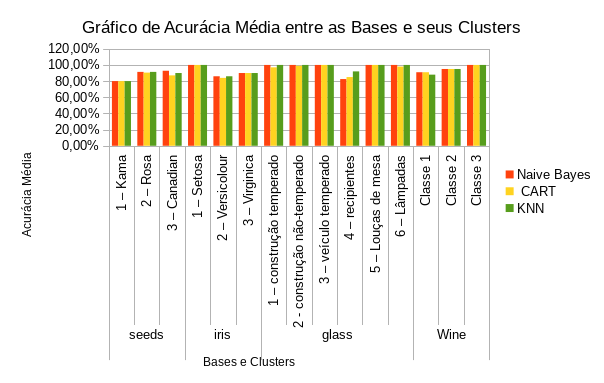
\includegraphics[scale=0.9]{figs/grafico_acuracia_media_algoritmos.png}
        \caption{Acurácia Média dos Rótulos dos Algoritmos: Naive Bayes, CART e KNN} \label{fig:acuracia_media_algoritmos}
\end{figure}

Uma breve análise do gráfico da figura \ref{fig:acuracia_media_algoritmos} referente as acurácias dos rótulos, fica claro que a qualidade deles foram satisfatórias, pois atingiram uma acurácia média com mínimo de 80\%. A acurácia desses rótulos servem para mostrar o quanto esses rótulos representam o grupo através das amostras testadas, e os três algoritmos tiveram acurácias bem parecidas, e em específico o Naive Bayes e KNN. Os clusters com menores acurácias 


